\documentclass[10pt,twocolumn,letterpaper]{article}

\usepackage{cvpr}
\usepackage{times}
\usepackage{epsfig}
\usepackage{graphicx}
\usepackage{amsmath}
\usepackage{amssymb}
\DeclareMathOperator*{\argmin}{arg\,min}

% Include other packages here, before hyperref.

% If you comment hyperref and then uncomment it, you should delete
% egpaper.aux before re-running latex.  (Or just hit 'q' on the first latex
% run, let it finish, and you should be clear).
\usepackage[breaklinks=true,bookmarks=false]{hyperref}

\cvprfinalcopy % *** Uncomment this line for the final submission

\def\cvprPaperID{****} % *** Enter the CVPR Paper ID here
\def\httilde{\mbox{\tt\raisebox{-.5ex}{\symbol{126}}}}

% Pages are numbered in submission mode, and unnumbered in camera-ready
%\ifcvprfinal\pagestyle{empty}\fi
\setcounter{page}{1}
\begin{document}

%%%%%%%%% TITLE
\title{Artistic Style Transfer}

\author{Suyan Qu\\
University of Wisconsin - Madison\\
Madison, WI 53706\\
{\tt\small squ27@wisc.edu}
}

\maketitle
%\thispagestyle{empty}

%%%%%%%%% ABSTRACT
\begin{abstract}
   Artistic style transfer is to apply the style of one image, the style image, typically a painting with special texture, to another image, the content image. The generated image will preserve the content presented in the content image while having the same style and texture of the style image. This project first demonstrates how to quantify the style and content difference between two images, through a pre-trained VGG19 model, which can be used to generate style transfered images through backpropogation, then presents a feed-forward deep network that can generate style-transfered images of size $300\times400$ in around $0.025$ seconds. 
\end{abstract}

%%%%%%%%% BODY TEXT
\section{Introduction}
For long, the style and content of a image are considered as two distinct aspects of a picture. People associate the content of an image with objects captured by the image while the style of the image with how the captured object is presented, such as the color scheme, the stroke, etc. Despite that, the style and content of an image are actually two integrated parts that cannot be physically separated. However, modern technology makes this task achievable. With the help of deep learning neural networks, it is possible to apply the style of famous paintings like starry night to a present-day photo, faking Van Gogh’s work in modern settings.
This technology can potentially accelerate the advancement of contemporary art, as it allows people with no previous experience in painting to create visually appealing images. This project aims to implement such style transfer system using convolutional neural networks. First, a pre-trained image classification model will be used to quantify the style and content difference between two images~\cite{Gatys}, which can be used to generate style transfered images through backpropogation, then a feed-forward transformation model will be implemented based on the style and content difference defined~\cite{Johnson}. 

%------------------------------------------------------------------------

\section{Related Work}

\subsection{VGG 19}
VGG 19 is a 19 layer convolutional neural network for large-scale image recognition~\cite{Simonyan} developped by Karen Simonyan and Andrew Zisserman in 2014. It can recognize images of 1000 different object categories. Its performance on ILSVRC-2012 dataset was remarkably well, with 23.7\% top 1 validation error and 6.8\% top 5 validation error. 

\subsection{Quantify Style and Content Difference}
In 2015, Leon A. Gatys, Alexander S. Ecker, and Matthias Bethge proposed a method that quantifies the style and content difference between two images with the assistant of a pretrained neural network~\cite{Gatys}. The basic intuition comes from the fact that shallower layers of an image classifier extract basic information of an input image, while deeper layers learn about the high level concepts that helps in classification. If two images have the same content, when they are sent into a image classifier, its deep layers should produce very similar results. Given two images, $x$ and $y$ and the output $X^l$ and $Y^l$ of a deep hidden layer $l$ of a pretrained network, content difference of these two images can be defined as
$$\mathcal{L}_{\text{content}}(x,y)=\frac{1}{2}\sum_{i,j}(X^l_{i,j}-Y^l_{i,j})^2$$
On the other hand, the style of an image may have influence in all layers. A good measure of style should capture the texture information but not the global arrangement. One such measure is the gram matrix. Given input images $x$ and $y$, and a hidden layer $l$ of a pretrained image classifier, define gram matrices $F^l$ and $G^l$ as
$$F^l_{i,j}=\sum_{k}X^l_{i,k}X^l_{j,k}$$
$$G^l_{i,j}=\sum_{k}Y^l_{i,k}Y^l_{j,k}$$
Then for each layer of dimension $N\times M$, a style difference $E_l$ can be calculated through
$$E_l=\frac{1}{4N^2_lM^2_l}\sum_{i,j}(F^l_{i,j}-G^l_{i,j})^2$$
With a chosen set of hidden layers $L$, the total style difference is the weighted sum of the style difference of each layer
$$\mathcal{L}_{\text{style}}(x,y)=\sum_{l\in L}w_lE_l$$

\subsection{Feed-Forward Transformation Network}
In recent years, various image transformation tasks have been trained with pixel-wise loss functions, such as semantic segmentation~\cite{Long}, depth and surface normal estimation~\cite{Eigen}, and etc. The feed-forward transformation model used in style transfer inspire from ~\cite{Long}, where downsampling is used to reduce the dimension of feature map, then upsampling is applied to produce the final result. 

\subsection{Instance Normalization}
In 2016, Ulyanov et al~\cite{Ulyanov2} point out that the result of stylization should not depend on the contrast of the content image in general as in batch normalization. In contrast, the style loss should be designed to transfer elements froma style image to the content image such that the contrast of the stylized image is similar to the contrast of the style image, and the general contrast of content images should be discarded. In another word, normalization should be specific to content images. In the recognition of this need, Ulyanov et al proposed instance normalization layer
$$y_{tijk}=\frac{x_{tijk}-\mu_i}{\sqrt{\sigma_i^2+\epsilon}}$$
$$\mu=\frac{1}{HW}\sum_{l=1}^W\sum_{m=1}^H x_{tilm}$$
$$\sigma^2_{ti}=\frac{1}{HW}\sum_{l=1}^W\sum_{m=1}^H(x_{tilm}-\mu_{ti})^2$$

\section{Method}
\subsection{Backpropogation with Loss Function}
Using the mechanism proposed by Gatys et al ~\cite{Gatys}, given a style image $s$, a content image $c$, and a generated image $g$, a loss function can be calculated as a weighted sum of the style loss between style image and generated image, and the content loss between the generated image and the content image
$$\mathcal{L}_{\text{total}}(s, c, g) = \alpha\mathcal{L}_{\text{content}}(c, g) + \beta\mathcal{L}_{\text{style}}(s, g)$$
With this loss function well defined, we can run an iterative algorithm similar to gradient descent on the generated image. During each iteration, the style, content, and generated images are sent into a pre-trained VGG 19 model. The $conv4\_2$ layer is used to calculate the content difference, which $conv1\_1$, $conv2\_1$, $conv3\_1$, $conv4\_1$, and $conv5\_1$ are used to calculate the style difference. With the loss function calculated, a gradient $\frac{\partial\mathcal{L}_{\text{total}}}{\partial g}$ can be calculated, and the generated image can be updated through gradient descent on the generated image
$$g'=g-\epsilon\text{sgn}(\frac{\partial\mathcal{L}_{\text{total}}}{\partial g})$$
Since it is harder to recover the content details than the style, the generated image in the first iteration is the same as the content image, except some random noises are added to break the original style and accelerate the process. It is also worth mention that max pooling layers are replaced by average pooling layers for better results. Some sample output are presented in figure 1
\begin{figure}[t]
\begin{center}
   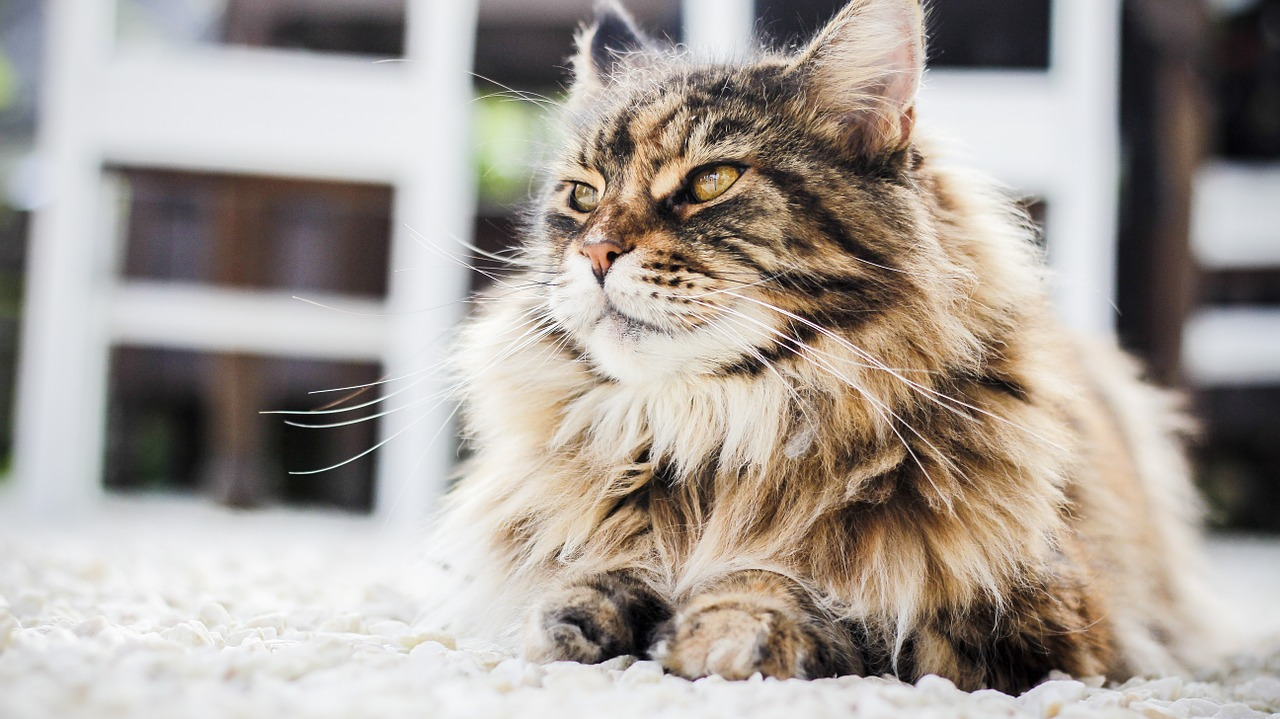
\includegraphics[width=0.45\linewidth]{persian_cat.jpg} 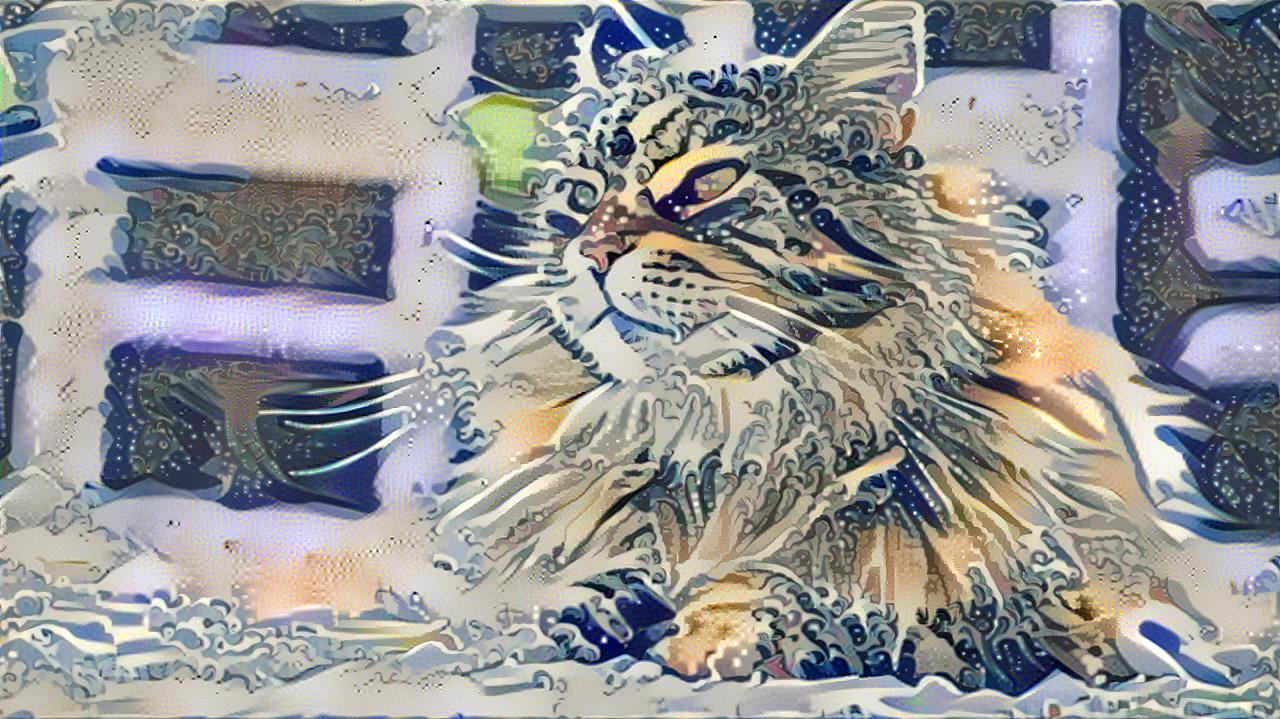
\includegraphics[width=0.45\linewidth]{persian_cat+hokusai.jpg}		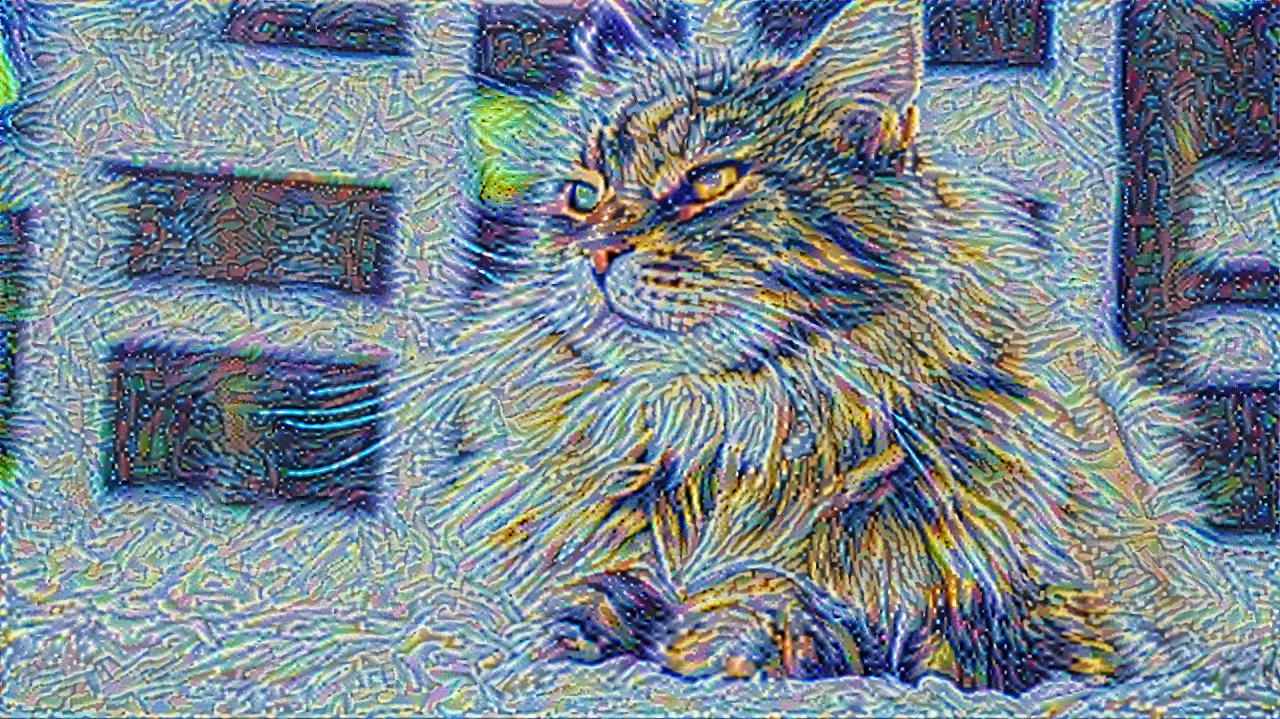
\includegraphics[width=0.45\linewidth]{persian_cat+starry_night.jpg} 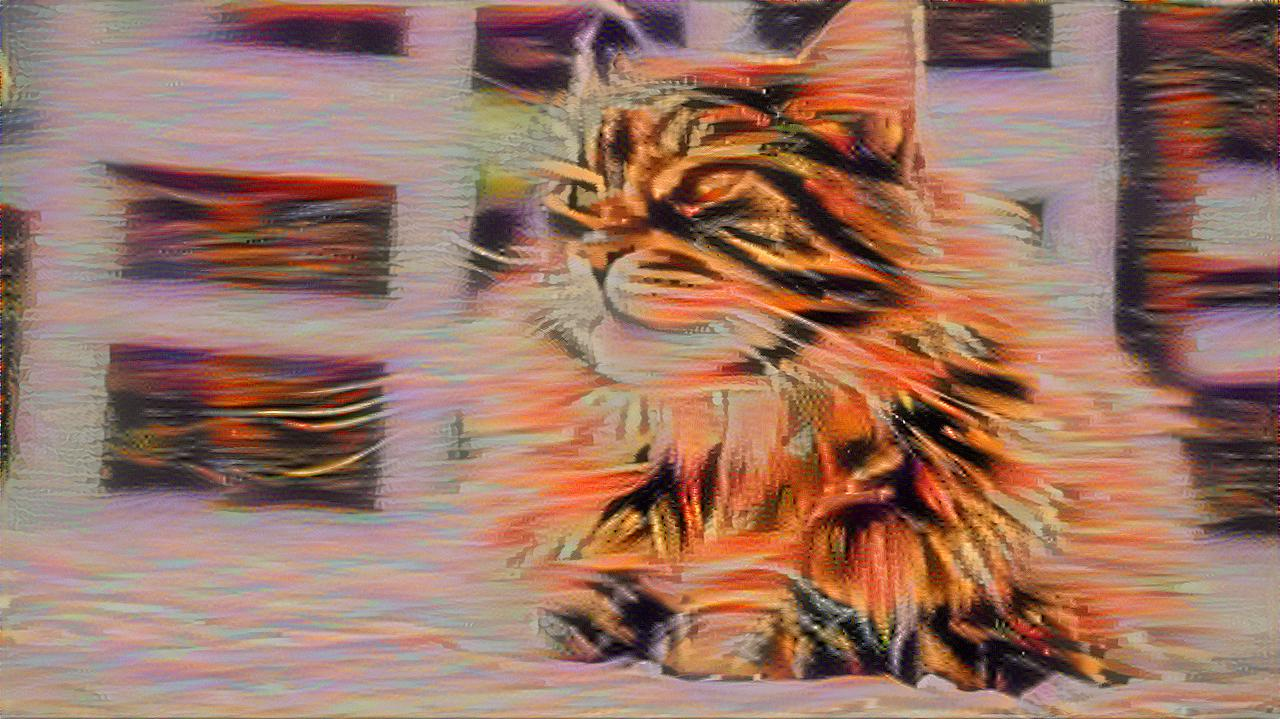
\includegraphics[width=0.45\linewidth]{persian_cat+the_scream.jpg}
\end{center}
   \caption{Sample outputs of the gradient descent approach. The upper left image is the original content image of a persian cat; the upper right is the original image styled with Hokusai; the lower left is the original image styled with Starry Night; the lower right is the original image styled with The Scream}
\label{fig:long}
\label{fig:onecol}
\end{figure}

\subsection{Texture Synthesis}
Gatys et al~\cite{Gatys2} also points out that the same algorithm can be used for texture synthesis. Texture synthesis, or texture extraction, is, as the name suggests, to generate a image with minor content but preserves the style of the original images. With the same algorithm above, a simple texture synthesis algorithm can be produced by running the backpropogation algorithm but replacing the content image with a blank image with noise. Some sample results are presented in figure 2.
\begin{figure}[t]
\begin{center}
   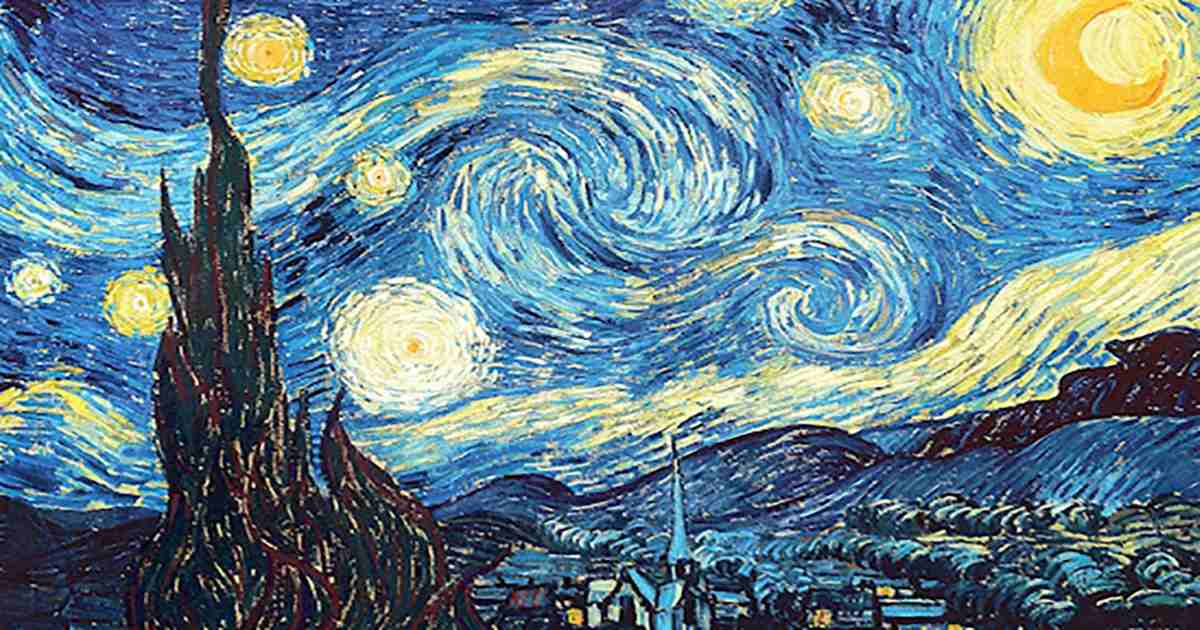
\includegraphics[width=0.45\linewidth]{starry_night.jpg} 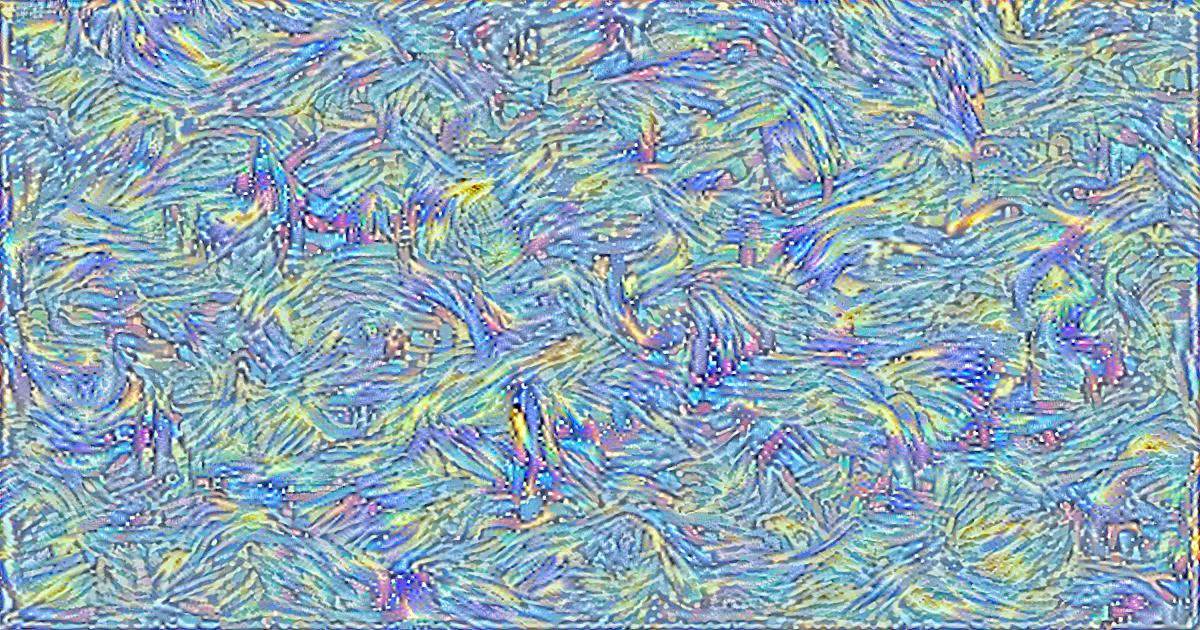
\includegraphics[width=0.45\linewidth]{starry_night_style.jpg}	
\end{center}
   \caption{Sample texture synthesis.The image on the left is the original image, Starry Night. On the right is the style synthesized from the texture synthesis algorithm}
\label{fig:long}
\label{fig:onecol}
\end{figure}

\subsection{Real-Time Style Transfer}
The backpropogation algorithm, as pointed out by Johnson et al~\cite{Johnson} and Ulyanov et al~\cite{Ulyanov}~\cite{Ulyanov2}, is extremely slow and inefficient. In practice, it takes, on a GTX 1050 ti, around 2 minutes to generate a $400\times 300$ image, while generating a high resolution $1200\times 900$ image can take 30 to 40 minutes. An alternative solution is to train a feed-forward transform network that takes in a content image and generates a stylized image. 
Such a model consists of two neural networks. A transform network $f_W$, that will transfer the content image to a stylized image, and a VGG19 model $\phi$, used to calculate $\mathcal{L}_{\text{total}}$. Given the content image $c$ and style image $s$, the generated image from this model would be $f_W(c)$. The loss function for training $f_W$ would be the same as defined before:
$$W=\argmin_{W}(\mathcal{L}_{\text{total}}(s, c, f_W(c)))$$
Notice that since the transform network takes in only the content image, the style image will be fixed druing training, so the trained model will be specific to the style of that image used in training. \\
Our transform network is similar to the network implemented by Johnson et al~\cite{Johnson} and Radford et al~\cite{Radford}, except that the batch normalization layers are replaced by the instance normalization layers proposed by Ulyanov et al~\cite{Ulyanov2} to produce better results. 

\section{Experiments and Results}
The model is trained on COCO 2014 train dataset~\cite{coco} for 1000 epochs. Figure 3 shows a sample output from this model. 
\begin{figure}[t]
\begin{center}
   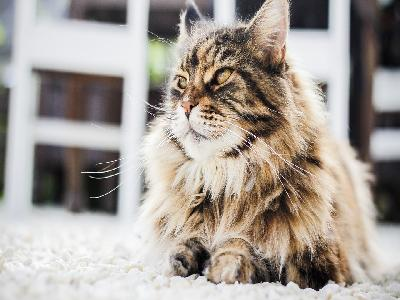
\includegraphics[width=0.45\linewidth]{input.jpg} 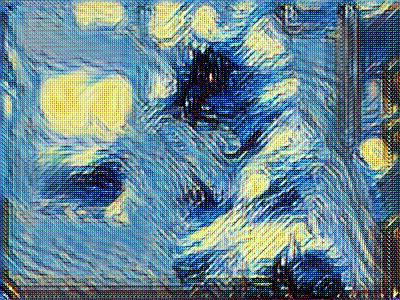
\includegraphics[width=0.45\linewidth]{generated_net.jpg}	
\end{center}
   \caption{Sample output of the transform network. On the left is the input image, and on the right is the input image stylized with Starry Night}
\label{fig:long}
\label{fig:onecol}
\end{figure}
As presented clearly from the sample output, the network does impressively well generating the style, but a lot of details of the content image are lost. One can only see the rough outline of the cat in the input image. In addition, when looking at the two windows to the left of the cat in the input image, which appears to be very dark, the window on bottom is stylized with dark blue texutres as expected, but the window on top is stylized with bright yellow textures. This unexpected and inconsistent shows that with random initialization, it is very hard to recover the content details compared with the texutre. To add more bias to the content difference, in addition to increasing the weight of $\mathcal{L}_{\text{content}}$ in calculating $\mathcal{L}_{\text{total}}$, some warmup epochs are applied. During warmup, the loss function is defined to be the difference between the direct output from the neural network and the input content image. In this way, the transform network is expected to be an identity model and should generate the exact same image as input before starting training. Result of the network with warmup is shown in figure 4. \\
\begin{figure}[t]
\begin{center}
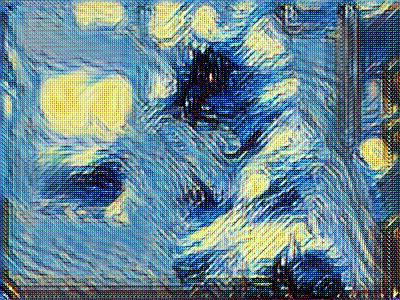
\includegraphics[width=0.45\linewidth]{generated_net.jpg} 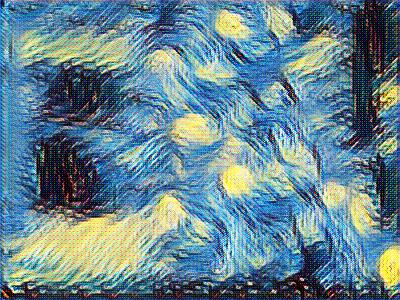
\includegraphics[width=0.45\linewidth]{generated_net_warmup.jpg}	
\end{center}
   \caption{On the left is the original output without warmup, and on the right is the output of the network trained with warmup. The same style and content image as in Figure 3 are used}
\label{fig:long}
\label{fig:onecol}
\end{figure}
As clearly seen in this direct comparison, the result generated with warmup has more consistencies. The black segments in the background are stylized with dark textures, while the white carpet and the white fur of the cat in foreground are stylized with bright yellow textures. It also preserves more of the content details. 

\subsection{Quantitative Results}
To evaluate the result of these models, the measure developed by Gatys et al~\cite{Gatys} will be adopted again. For a content image $c$, a style image $s$, and a image generated from the model $g$, we will calculate $\mathcal{L}_{\text{content}}(g, c)$, which quantifies the content difference between content image and generated image, and $\mathcal{L}_{\text{style}}(g, s)$, which quantifies the style difference between style image and generated image. The smaller $\mathcal{L}_{\text{content}}(g, c)$ is, better the model preserves the content. The smaller $\mathcal{L}_{\text{style}}(g, s)$ is, the better the model stylizes the image. Table 1 shows these measures for the backpropogation model, the transform network without warmup, and the transform network with warmup. The table shows that the naive backpropoation method does impressively better than using transform network both in terms of style difference and content difference, and the use of warmup epochs effectively reduces the content difference by 8.4\%, and reduces the style difference to only 11.6\% of the original difference, which is kind of counter intuitive, as the warmup epochs are designed to improve the content difference. \\

\begin{table}
\begin{center}
\begin{tabular}{|l|c|c|}
\hline
Model & $\mathcal{L}_{\text{content}}$ & $\mathcal{L}_{\text{content}}$ \\
\hline\hline
Back-Prop & 32143.725 & 2679063.8\\
Transform Net & 46208.43 & 622746200.0\\
Transform Net + Warmup & 42328.656 & 72501340.0\\
\hline
\end{tabular}
\end{center}
\caption{Style and Content Difference using Different Approaches}
\end{table}

Another Measure that worths notice is the runtime for these 2 methods, as shown in table 2. A transform network only need 0.025 seconds to transform a $400\times 300$ image, which is $1081$ times faster than the backpropogation method. Compared with the iterative gradient descent method, this method only requires a single pass of the input image into the network. 
\begin{table}
\begin{center}
\begin{tabular}{|l|c|}
\hline
Model & Runtime \\
\hline\hline
Back-Prop 400 Iteration & 27.03s\\
Transform Net & 0.026s\\
Transform Net + Warmup & 0.025s\\
\hline
\end{tabular}
\end{center}
\caption{Runtime for $400\times 300$ Images Using Different Model on Tesla K80}
\end{table}

\section{Conclusion}
In this project, we implemented the gradient descent algorithm proposed by Gatys et al~\cite{Gatys} and the feed-forward transform network proposed by Johnson et al~\cite{Johnson} with some improvements including replacing the batch normalization layers by instance normalization~\cite{Ulyanov2} and warmup epochs. The results generative are impressive, but are not exactly what we expected. The output image from the transform network is of low resolution and many content details are lost. Figure 5 shows the output after the warmup epochs and one training epoch, implying that the content details may have lost during upsamplying and downsampling in the first place. \\
Future explorations will be focusing on how to preserve more of the details of a content image in the transform network, including how to improve the resolution of the output. We will also try some different network architextures for this task to see their result. 

\begin{figure}[t]
\begin{center}
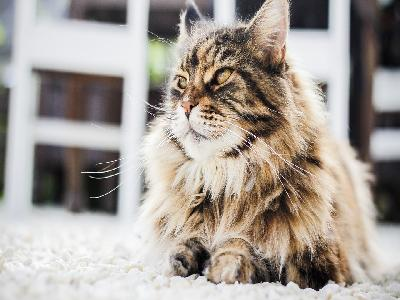
\includegraphics[width=0.45\linewidth]{input.jpg} 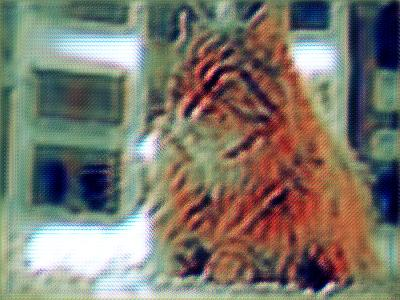
\includegraphics[width=0.45\linewidth]{0.jpg}	
\end{center}
   \caption{The output of transform network after warmup}
\label{fig:long}
\label{fig:onecol}
\end{figure}
{\small
\bibliographystyle{ieee_fullname}
\bibliography{egbib}
}

\end{document}
